% begin module trig-functions
\begin{frame}
\frametitle{The Trigonometric Functions}
\[
\begin{array}{|cc|cc|}
\hline
\multicolumn{2}{|c|}{%
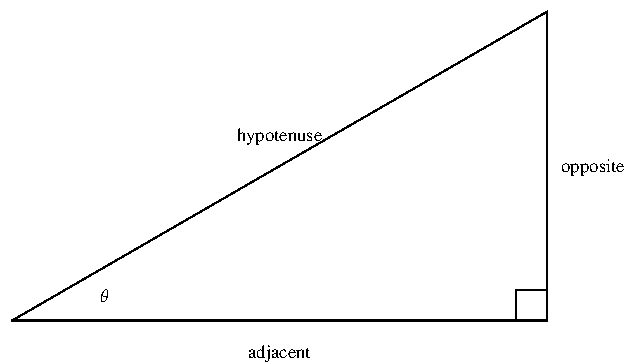
\includegraphics[width=5cm]{trigonometry/pictures/app-d-ratiosa.pdf}%
}&%
\multicolumn{2}{|c|}{%
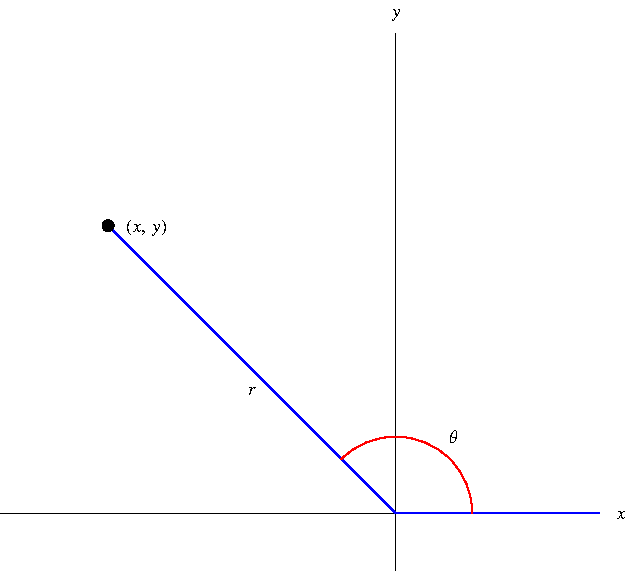
\includegraphics[width=5cm]{trigonometry/pictures/app-d-ratiosb.pdf}%
}\\%
\sin \theta = \frac{\textrm{opp}}{\textrm{hyp}} &
\csc \theta = \frac{\textrm{hyp}}{\textrm{opp}} &
\sin \theta = \frac{ y}{ r} &
\csc \theta = \frac{ r}{ y} \\
\cos \theta = \frac{\textrm{adj}}{\textrm{hyp}} &
\sec \theta = \frac{\textrm{hyp}}{\textrm{adj}} &
\cos \theta = \frac{ x}{ r} &
\sec \theta = \frac{ r}{ x} \\
\tan \theta = \frac{\textrm{opp}}{\textrm{adj}} &
\cot \theta = \frac{\textrm{adj}}{\textrm{opp}} &
\tan \theta = \frac{ y}{ x} &
\cot \theta = \frac{ x}{ y} \\
\hline
\multicolumn{2}{|c|}{\textrm{Acute angles}}&
\multicolumn{2}{|c|}{\textrm{Obtuse or negative angles}}\\
\hline
\end{array}
\]
\end{frame}
% end module trig-functions
